\begin{figure}[ht]
\centering
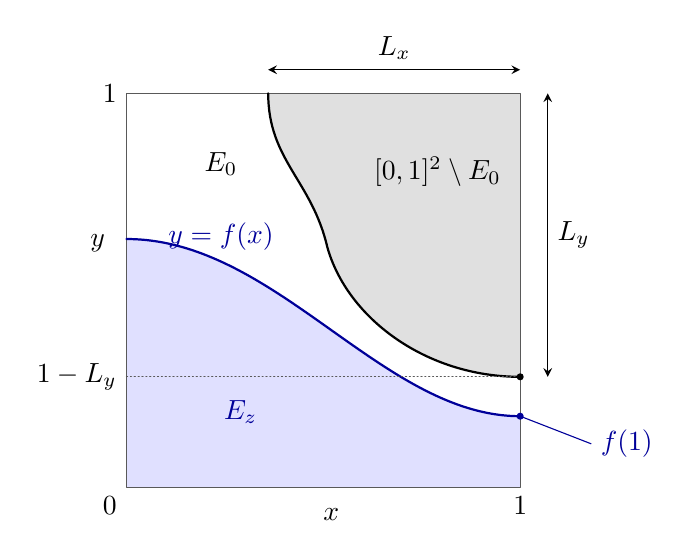
\begin{tikzpicture}[x=5cm,y=5cm,>=stealth,line cap=round,line join=round]
 \fill[black!12] (0.36,1) -- (1,1) -- (1,0.28)
   .. controls (0.76,0.28) and (0.56,0.43) .. (0.51,0.61)
   .. controls (0.47,0.78) and (0.36,0.83) .. (0.36,1) -- cycle;
 \fill[blue!12] (0,0) -- (1,0) -- (1,0.18)
   .. controls (0.65,0.18) and (0.38,0.63) .. (0,0.63) -- cycle;
 \draw[black!65] (0,0) rectangle (1,1);
 \draw[thick] (0.36,1)
   .. controls (0.36,0.83) and (0.47,0.78) .. (0.51,0.61)
   .. controls (0.56,0.43) and (0.76,0.28) .. (1,0.28);
 \draw[thick,blue!60!black] (0,0.63)
   .. controls (0.38,0.63) and (0.65,0.18) .. (1,0.18);
 \draw[<->] (0.36,1.06) -- node[above] {$L_x$} (1,1.06);
 \draw[<->] (1.07,0.28) -- node[right] {$L_y$} (1.07,1);
 \draw[densely dotted,black!65] (0,0.28) -- (1,0.28);
 \node[left] at (0,0.28) {$1-L_y$};
 \fill (1,0.28) circle[radius=0.009];
 \fill[blue!60!black] (1,0.18) circle[radius=0.009];
 \draw[blue!60!black] (1,0.18) -- (1.18,0.11);
 \node[right,blue!60!black] at (1.18,0.11) {$f(1)$};
 \node at (0.79,0.80) {$[0,1]^2\setminus E_0$};
 \node[blue!60!black] at (0.29,0.19) {$E_z$};
 \node at (0.24,0.82) {$E_0$};
 \node[blue!60!black,above] at (0.24,0.575) {$y=f(x)$};
 \node[below left] at (0,0) {$0$};
 \node[below] at (1,0) {$1$};
 \node[left] at (0,1) {$1$};
 \node[below] at (0.52,-0.03) {$x$};
 \node[left] at (-0.03,0.62) {$y$};
\end{tikzpicture}
\caption{Nesting constrains a strip through the bottom complement.
The shaded strip $E_z=\{(x,y):0\leq y\leq f(x)\}$ lies in $E_0$,
so its smaller endpoint satisfies $f(1)\leq1-L_y$.
Interchanging $x$ and $y$ gives the bound using $L_x$ for the other
strip orientation. The curves and the unequal extents are schematic;
no convexity or circular shape is assumed.}
\label{nest:containment-figure}
\end{figure}
